\chapter{\label{chapter1} Parton distribution functions} 
Parton distributions are one of the central pillars of perturbative QCD, factorising as they do the perturbatively incalculable long distance dynamics present in calculations involving hadronic initial states. Combined with
the perturbative description of the short-distance cross-section what could seem at first a hopeless situation is alleviated, and QCD becomes a predictive and useful theory when applied to hadronic scattering.

In this chapter a brief overview of how parton distribution functions arise in QCD calculations will be presented.
We shall explore the prototypical example of the deep inelastic scattering (DIS) of leptons off a hadronic target, first in the \emph{naive parton model} arising before the advent of QCD and then with the QCD-improved parton model which allows for an excellent description of DIS measurements across a wide range of hard scales.

The treatment of heavy quarks in parton distributions is a particularly delicate issue and therefore will
also be discussed in this introductory theory section. Finally there will be some exploration of the general properties of parton distributions in order to provide a summary of the available theoretical constraints upon PDFs.

\section{Partons in deep inelastic scattering}
We shall begin by introducing parton distribution functions as they arise in the early parton model. The model was originally introduced by Feynman and Bjorken~\cite{feynman1,Feynmanparton,feynmanparton2, Bjorken:1968dy} in the late 1960's in an effort to understand the scattering behaviour of hadronic states and successfully
describes many properties observed in early deep inelastic scattering experiments.

In this process, a charged lepton $l$ probes a proton $P$ by the exchange of a gauge boson. For simplicity we shall describe here the neutral current process where a photon is exchanged. In the inelastic regime where the momentum transfer to the target proton is large, the proton does
not survive the scattering process and fragments into an arbitrary hadronic final state $X$. The process $l(k) + P(p) \to l(k^\prime) + X$ is illustrated at tree level in Figure \ref{fig:DIS}. 

\begin{figure}[ht]
\centering
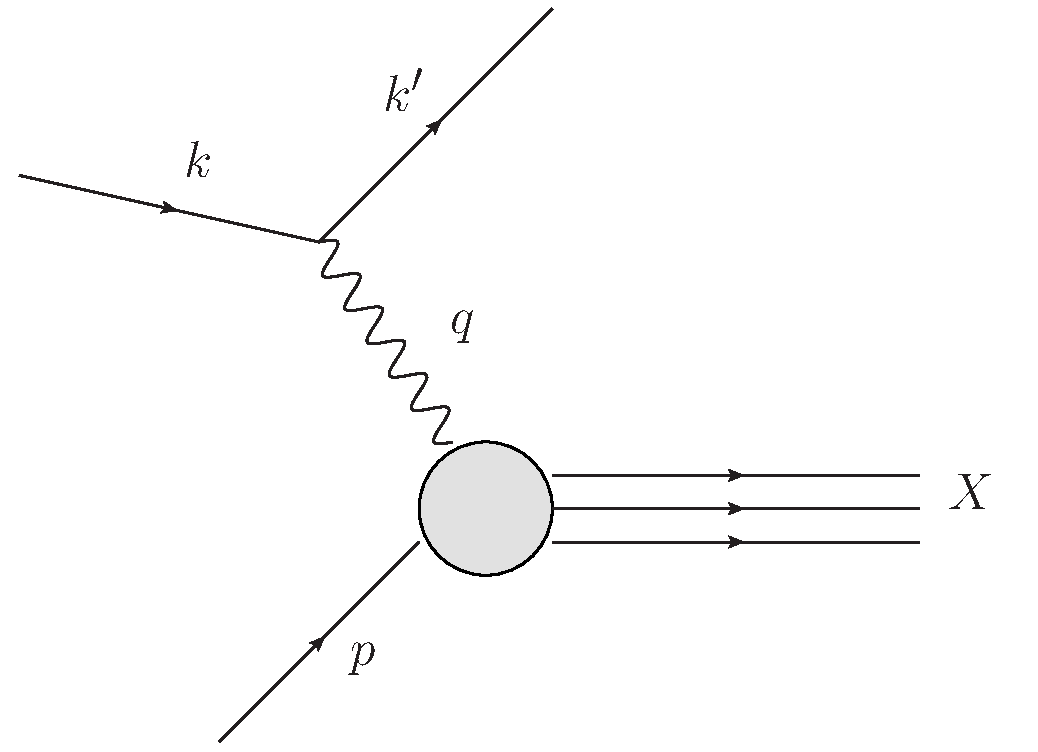
\includegraphics[scale=0.5]{2-PDFs/figs/DIS.pdf}
\caption{Deep inelastic scattering of a charged lepton with a proton target.}
\label{fig:DIS}
\end{figure}

In this system we can define the standard DIS kinematic variables;  $Q^2$ denotes the momentum transfer from the electron to the target proton, $\nu$ the energy transfer and $y$ the measure of the reaction's inelasticity, or fractional energy transfer. In the rest frame of the proton these are given by
\begin{eqnarray}
 Q^2 &=& -q^2 = -(k - k^{\prime})^2, \\
 \nu &=& M(E- E^\prime), \\
 y &=& (q \cdot p)/(k \cdot p),
\end{eqnarray}
where $M$ refers to the mass of the proton, and the inelasticity ranges between 0 (elastic scattering) and 1. $E$ and $E^\prime$ denote the energies associated with the four-momenta $k$ and $k^\prime$ respectively. Additionally, we may introduce the Bjorken scaling parameter $x$, central to the parton model,
\be x = \frac{Q^2}{2\nu}. \ee
Neglecting spin labels, the amplitude for this diagram in the Feynman gauge is given by
\be\mathcal{M} = ie^2\bar{u}(k^\prime)\gamma^\mu u(k)\left( i\frac{g_{\mu\nu}}{Q^2} \right)\left<X\right|J_h^\nu\left|P\right>,  \label{eq:DISme}\ee
where $J_h^\nu$ represents the hadronic current. 
The fundamental difficulty in attempting to compute the cross section for this process is our ignorance of the wavefunction for the hadronic states $\left|X\right>$ and $\left|P\right>$. To isolate the problem, we are able to factorise the spin averaged square of the amplitude in Equation \ref{eq:DISme} into a leptonic ($L_{\mu\nu}$) and a hadronic ($W^{\mu\nu}$) part
\be |\overline{\mathcal M}|^2 = \frac{1}{Q^2} L_{\mu\nu}W^{\mu\nu}, \ee
where the leptonic tensor is straightforwardly calculable:
\ba L_{\mu\nu} &=& e^2\sum_{spin} \bar{u}(k^\prime)\gamma_\mu u(k) \bar{u}(k)\gamma_\nu u(k^\prime), \\
&=& e^2 \mathrm{ tr}\left[ \slashed{k}^\prime\gamma_\mu\slashed{k}\gamma_\nu \right], \\
&=& 4e^2[k_\mu k^\prime_\nu + k_\nu k^\prime_\mu - g_{\mu\nu}k\cdot k^\prime],  \ea
where here we have neglected the fermion masses. The hadronic part of the calculation is considerably more difficult to evaluate, and indeed impossible to compute from first principles in perturbation theory as it is sensitive to the low-scale, and therefore strongly coupled dynamics of the proton target:
\ba  
W^{\mu\nu} &\sim& \sum_X \left<P(p)\right| {J_h^\mu}^{\dagger} \left|X\right>\left<X\right| J_h^\nu \left| P(p)\right>, \\
 &\sim& \left<P(p)\right| {J_h^\mu}^{\dagger} J_h^\nu \left| P(p)\right>. \ea

However, we can gain some insight into its structure by noting that the tensor must obey the conservation requirements of the hadronic current $q_\mu W^{\mu\nu}=0$ and $q_\nu W^{\mu\nu}=0$. The tensor may therefore be parametrised without loss of generality by the following structure:
\be W_{\mu\nu} = -\left( g_{\mu\nu} - \frac{q_\mu q_\nu}{q^2}\right) F_1(x,Q^2) +\left(p_\mu -q_\mu \frac{p \cdot q}{q^2}\right)\left(p_\nu -q_\nu \frac{p \cdot q}{q^2}\right)\frac{1}{\nu}F_2(x,Q^2).\label{eq:htensor}\ee
Here we have introduced the parameters in our tensor $F_i$ which are known as the electromagnetic structure functions. For interactions involving parity-violating currents, there is a third contribution to the hadronic tensor arising through the $F_3$ structure function. Here the only possible functional dependence for the structure functions is upon the quantities $Q^2$ and $x$.

It is convenient now to define a projection vector $n$ with the properties $ p \cdot n = 1$, $ n \cdot q = 0$, and $n^2 = p^2 = 0$, where the assumption of negligible proton mass has been made. Any vector can now be written as a combination of $n$, $p$ and a component transverse to the proton momentum as a \emph{Sudakov decomposition}. Using this projection vector we may obtain the structure functions from the hadronic tensor as so:
\begin{eqnarray}
 F_2 &=& \nu n^\mu n^\nu W_{\mu\nu},  \label{eq:proj1} \\
 F_L &=& F_2 - 2xF_1 = \frac{Q^4}{\nu^3}  p^\mu p^\nu W_{\mu\nu}, \label{eq:proj2}
\end{eqnarray}
where the quantity in the second equation is known as the longitudinal structure function. So far, few assumptions have been made about the form of the EM hadronic tensor $W_{\mu\nu}$, we have simply parametrised it in terms of a Lorentz invariant tensor structure and structure functions. Feynman's parton model allows us to describe more of the hadronic tensor with perturbation theory by proposing a composite proton formed as a bound state of fundamental, spin-$1/2$ constituents: the \emph{partons}. 

The parton model approximation states that for a sufficiently hard interaction, the virtual photon only interacts with a single point-like parton inside the target proton and we can treat the partons as approximately free particles. The hadronic tensor then admits a probabilistic expansion in terms of Parton Distributions which encode the probability of the hard photon interacting with a constituent parton carrying a faction $\xi$ of the parent proton's momentum. The probability of interacting with a parton carrying between $\xi$ and $\xi+\delta\xi$ of the proton's momentum being given by $f(\xi)\delta\xi$ where $f(\xi)$ is the interaction probability for a parton with momentum $\xi p$. Diagrammatically we may therefore construct the photon-hadron interaction as a weighted sum of partonic diagrams:
\be \left| \vcenter{\hbox{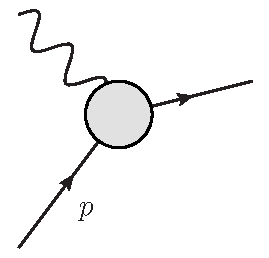
\includegraphics[height=2cm]{2-PDFs/figs/convolution1.pdf}}} \right|^2= \sum_i^{N_{part}}f_i(\xi,Q^2) \otimes \left| \vcenter{\hbox{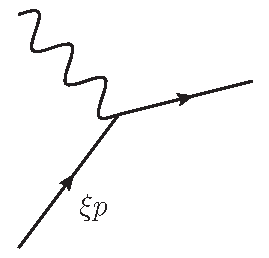
\includegraphics[height=2cm]{2-PDFs/figs/convolution2.pdf}}}\right|^2(\xi), \nonumber\ee
where we have introduced the multiplicative convolution
\be (f \otimes g )(x) = \int_0^1\; \frac{d\xi}{\xi}\; f\left(\frac{\xi}{x}\right) g(\xi).\ee
The hadronic tensor is then given in terms of a sum of individual hard scattering partonic tensors, denoted  $\widetilde{W}^i_{\mu\nu}(\xi)$ for a target parton of type $i$. Writing the hadronic tensor as the probabilistic sum over all constituent parton types we obtain
\be W_{\mu\nu} =\int_0^1 \frac{d\xi}{\xi} \sum_i f_i(\xi,Q^2)\; \widetilde{W}^i_{\mu\nu}(\xi,Q^2). \label{eq:htensorexpan}\ee
As the parton level tensors must obey the same conservation relations as the full hadronic tensor, we can once again form a general parameterization of $\widetilde{W}^i_{\mu\nu}$:
\be \widetilde{W}^i_{\mu\nu} = -\left( g_{\mu\nu} - \frac{q_\mu q_\nu}{q^2}\right) \widetilde{F_1^i}(\xi,Q^2) +\xi^2 \left(p_\mu -q_\mu \frac{p \cdot q}{q^2}\right)\left(p_\nu -q_\nu \frac{p \cdot q}{q^2}\right)\widetilde{F_2^i}(\xi,Q^2),\ee
where the factors of $\xi^2$ arise from taking $p^\mu \to \xi p^\mu$. Substituting this form for $\widetilde{W}^i_{\mu\nu}(\xi)$ into Eqn \ref{eq:htensorexpan} and comparing with the form in Eqn \ref{eq:htensor}, we find two expressions for the proton EM structure functions,
\be F_1(x,Q^2) = \int_0^1 \frac{d\xi}{\xi} \sum_i f_i(\xi) \widetilde{F_1^i}(\xi,Q^2),  \label{eqn:f1}\ee
\be F_2(x,Q^2) = \int_0^1 \xi d\xi \sum_i f_i(\xi) \widetilde{F_2^i}(\xi,Q^2). \label{eqn:f2}\ee
The naive parton level structure functions $\widetilde{F_1^i}(\xi,Q^2)$ describe the hard scattering subprocess involving a parton of species $i$ and may be computed by considering the parton level squared amplitude for the subprocess, $\gamma^*(q) + q(\xi p) \to q(l)$ and projecting out the desired quantities with the operators defined previously. At leading order, using the parton level version of the projector Eqn \ref{eq:proj1}:
\be { \mathcal M }_\mu = -i e_{q^i}\bar{u}(l)\gamma^\mu u(\xi p),\ee
\be \frac{n^\mu n^\nu}{\xi^2} \widetilde{W}^i_{\mu\nu}  = \frac{n^\mu n^\nu}{\xi^2}\overline{\sum} \left| \mathcal{M} \right|^2_{\mu\nu} = 4e_{q^i}^2,\ee
where we have made the approximation that momenta transverse to the beam axis vanish. Including the phase space for the final state quark in the CM frame we obtain:
\be \widetilde{F^i_2} =  2 e_{q^i}^2 \delta(l^2),\ee
where the delta function can be rewritten in terms of $\xi p$ and $q$:
\be \delta (l^2) = \delta ((\xi p + q )^2 ) = \delta (2\xi \nu - Q^2) = \delta (2\nu (\xi - x)).\ee 
This is an interesting result of the analysis at leading order, the kinematical variable $x$ actually describes the momentum fraction of the interacting parton. The parton level structure function
$\widetilde{F^i_2}$ is therefore given by:
\be \widetilde{F^i_2} = 2 e_{q^i}^2 \delta (\xi-x).\ee
The parton level longitudinal structure function is also straightforwardly projected out of the same amplitude,
\be \widetilde{F}^i_L = \frac{Q^4}{\xi \nu^3}p^\mu p^\nu \widetilde{W}^i_{\mu\nu} =  \widetilde{F}^i_2 - \frac{2x}{\xi^2} \widetilde{F}^i_1. \ee
At leading order this projection, and therefore the longitudinal structure function, are exactly zero, consequently
\be \widetilde{F}^i_1 = \frac{\xi^2}{2x} \widetilde{F}^i_2 = e_{q^i}^2\frac{ \xi^2 }{x} \delta (\xi - x).\ee
We may therefore write the full EM proton structure functions in the naive parton model as
\be F_1(x,Q^2) =  \int_0^1 d\xi \sum_i f_i(\xi) e_{q^i}^2\frac{ \xi }{x} \delta (\xi - x) =  \sum_if_i(x)e^2_{q^i},\ee
\be F_2(x,Q^2) = 2 \int_0^1 \xi d\xi \sum_i  f_i(\xi) e_{q^i}^2 \delta (\xi-x) = 2 x \sum_if_i(x)e^2_{q^i}.\ee
These results have a number of important features. Firstly in this model the structure functions have no dependence upon the resolution parameter $Q^2$, a phenomenon known as Bjorken scaling~\cite{Bjorken:1968dy}. This scaling effect was an important achievement of the original parton model, as it was able to describe contemporary experimental results rather well. The lack of any scale dependence in the structure functions is a consequence of the model's assumptions treating interactions with the proton's constituent partons as point like, and consequently having no characteristic length scale.

Secondly we note that $F_2(x) = 2xF_1(x)$, which is known as the Callan-Gross relation~\cite{callangross}. It illustrates a fundamental property of spin-1/2 particles, that they are unable to absorb a longitudinally polarised photon~\cite{pQCDhandbook}.
%
\section{QCD and the parton model}
The naive parton model was able to provide a good phenomenological description of early DIS measurements. Its success also provided great support for QCD as the correct description of the strong interaction. The phenomenon of Bjorken scaling placed substantial constraints upon the theory governing the internal dynamics of the proton. The asymptotic freedom of QCD allows for a consistent description of Bjorken-scaling, where the constituents of the hadron can be viewed as independent, non-interacting point like particles at high  values of the resolution parameter $Q^2$. The partons in Feynman's model were therefore quickly associated with the quarks and gluons of QCD.
\begin{figure}[t]
\centering
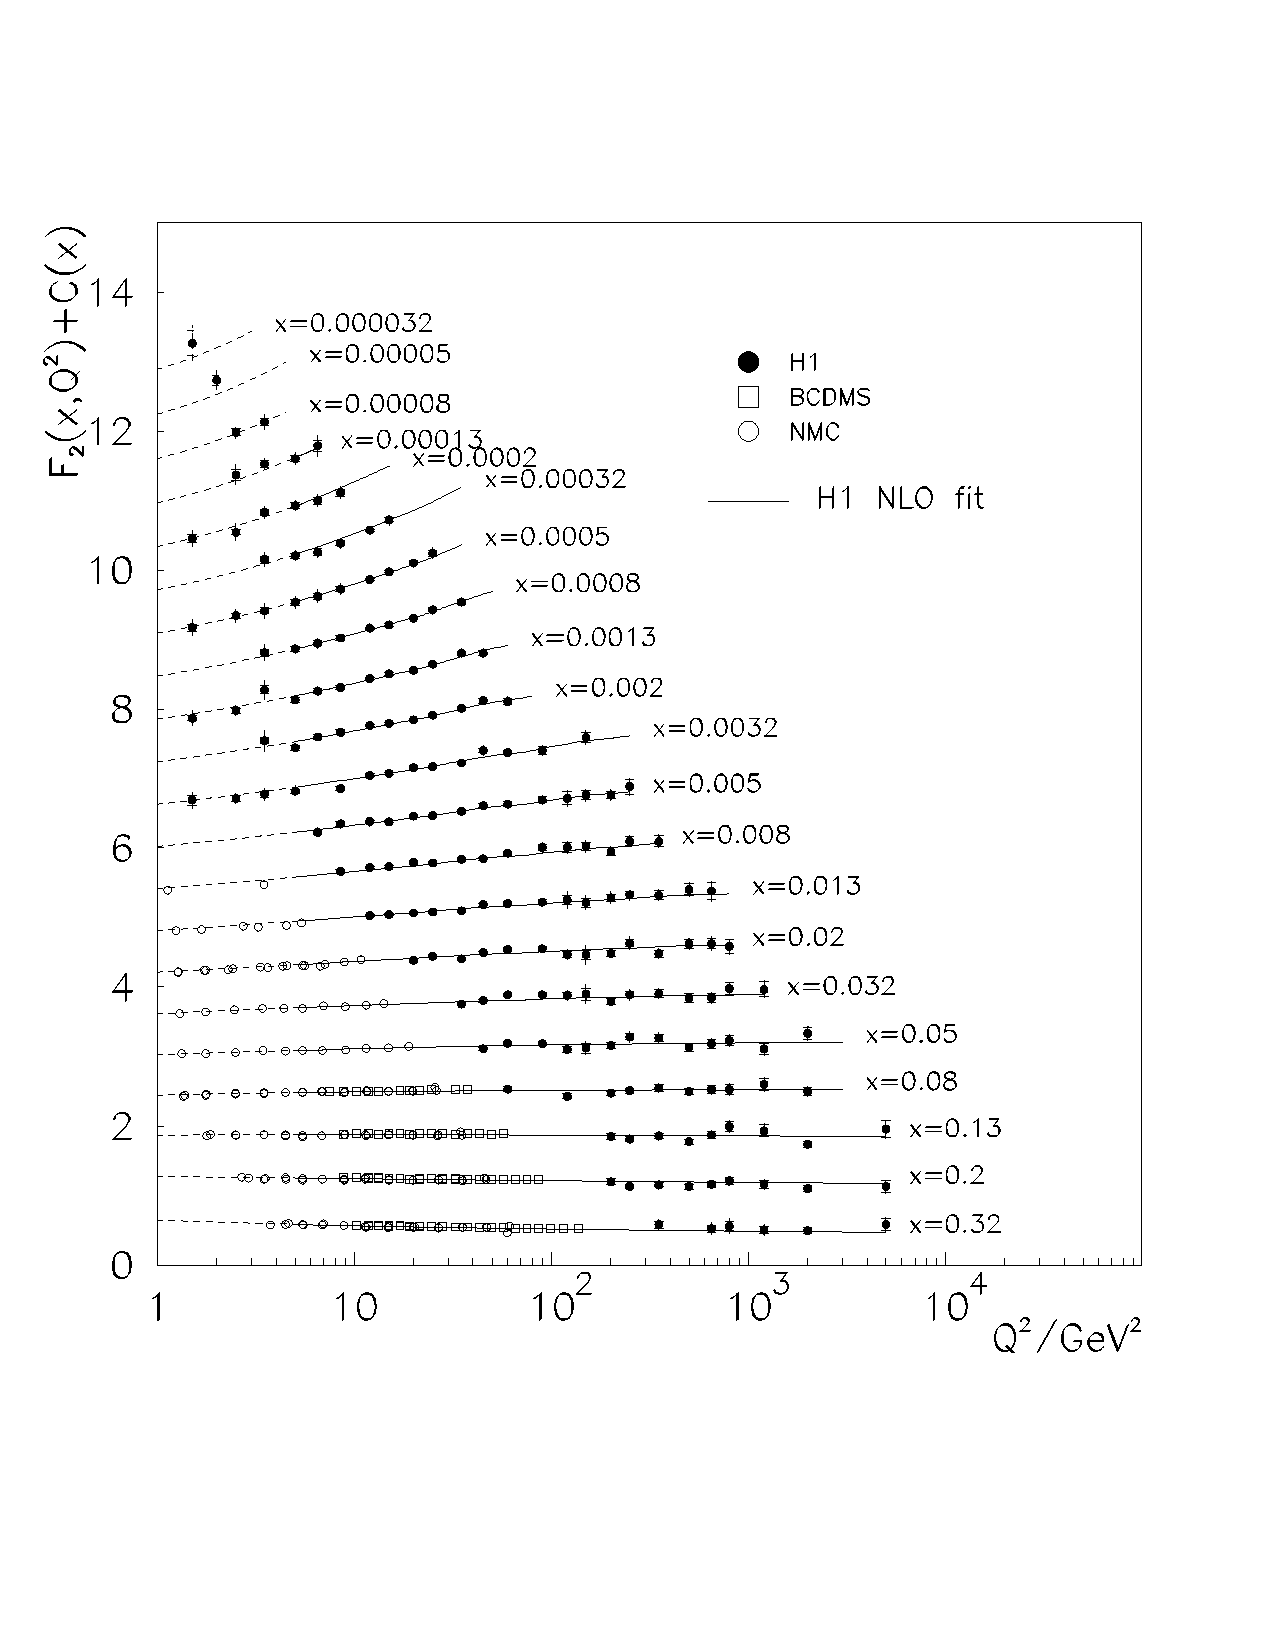
\includegraphics[scale=0.5]{2-PDFs/figs/d96-039f11.pdf}
\caption[Scaling violations in the proton structure function $F_2$]{Scaling violations in the proton structure function $F_2$. Here each curve in $x$ is scaled by a function $C(x)= 0.6(i- 0.4)$ for presentation purposes, where $i$ denotes the bin in $x$. Figure from~\cite{Aid:1996au}.}
\label{fig:F2H1}
\end{figure}

Despite the `snapshot' picture of non-interacting partons at leading order in QCD, we cannot neglect the higher order corrections to the point vertex calculated in the previous section. These corrections introduce logarithms of $Q^2$ which break the naive Bjorken scaling of the structure functions. Indeed, the measurement of such scaling violations provided one of the most powerful experimental verifications of QCD. Such violations are demonstrated in measurements of $F_2$ in Figure \ref{fig:F2H1}. In this section we shall perform an overview of the extension of the parton model to $\mathcal{O}(\alpha_s)$ in QCD.

At one loop order, there are three diagrams that contribute to the $qq\gamma$ vertex studied in the previous section; the real emission of a gluon from the initial (a) or final state (b) quarks, and the virtual correction diagram (c). Additionally at one loop order in QCD there arises a diagram initiated by a gluon splitting into a $q\bar{q}$ pair (d).

\begin{figure}[ht]
\centering
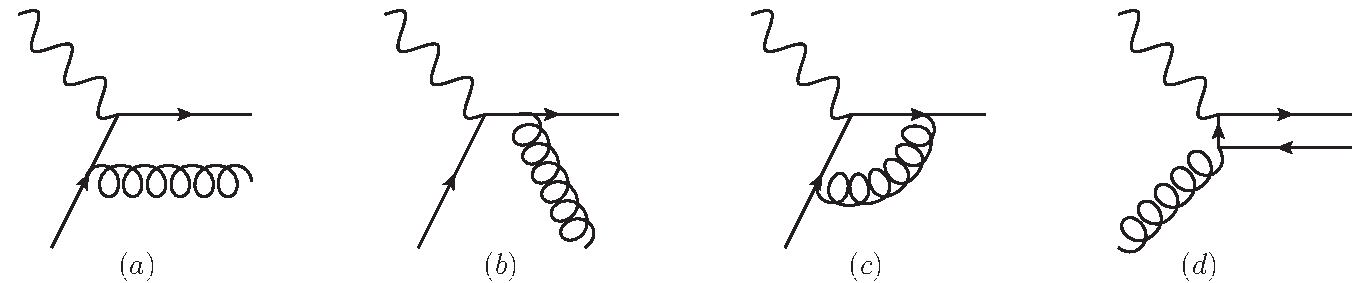
\includegraphics[scale=0.6]{2-PDFs/figs/1loopDIS.pdf}
\end{figure}

All four of these diagrams are separately divergent. When appropriately regularised however, the divergences in the final state real emission and virtual correction diagrams cancel explicitly as a consequence of the IR safety of QCD, yielding a finite contribution to the cross section. However the divergences present in the real emission diagrams from the initial state partons are not subject to the same cancellations, as they modify the momenta at the interaction vertex. 
 
Like the real emission diagram of a gluon from an initial state quark, the initial state gluon diagram (d) suffers from an equivalent divergence mediated by a perturbatively calculable $g\to q\bar{q}$ splitting function $P_{gq}$. Including all of the finite contributions from the other contributing diagrams as the coefficient $W(x)$, the parton level structure function at next to leading order in QCD is given by
\ba
 \widetilde{F_2^i}(\xi,Q^2) &=& 2 e_i^2\left[ \delta(\xi-x) \right. \nonumber\\
 				 &+& \frac{\alpha_S}{2\pi}\sum_j\left(P_{ij}(\xi)\log\frac{Q^2}{\kappa^2} + W_{ij}(\xi)\right) \nonumber\\
				 &+&  \left. \mathcal{O}(\alpha_S^2) \right]. \label{eq:f2plnlo}
\ea
Here the $i$ once again refers to the partonic species at the interaction vertex, and we have introduced an infrared cutoff $\kappa$ to regulate the parton splitting. The sum over splitting functions arises from the multiple contributions from partonic species $j$ splitting to $i$:
\begin{figure}[ht]
\centering
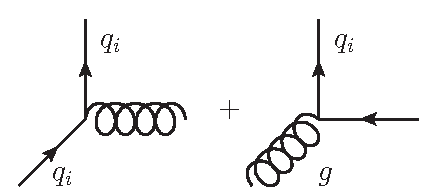
\includegraphics[scale=0.6]{2-PDFs/figs/qgq.pdf}
\end{figure}

The splitting functions $P_{ij}$  were known for some time at leading and next-to-leading accuracy \cite{Gross:1973ju,Georgi:1951sr,Floratos:1977au,Altarelli:1977zs,GonzalezArroyo:1979df,Floratos:1978ny,Furmanski:1980cm,Curci:1980uw,GonzalezArroyo:1979he,Floratos:1981hs,Hamberg:1991qt}, and more recently extended to next-next-to-leading order accuracy \cite{Moch:2004pa,Vogt:2004mw}. After convoluting the parton level functions with the PDFs, we obtain the full structure function 
\ba
 F_2(x,Q^2) &=& \sum_i xe_i^2\left[\; f_i(x) \right.  \nonumber\\
 				 &+& \frac{\alpha_S}{2\pi}\int_0^1 \frac{d\xi}{\xi}\sum_j\left(P_{ij}\left(\frac{x}{\xi}\right)\log\frac{Q^2}{\kappa^2} + W_{ij}(x)\right)\; f_j(\xi) \nonumber \\
				 &+&  \left. \mathcal{O}(\alpha_S^2) \right]. \label{eq:f2nlo}
\ea
Our expression for the parton level structure function still suffers from the IR divergence when we take the limit $\kappa\to 0$. This issue may be resolved by concluding that the singularity arises from a breakdown of the ability of perturbation theory to describe physics in the strongly-coupled infrared. We may therefore attempt to factorise out the long distance behaviour of the structure functions into some bare parameters of the theory; analogously to the treatment of ultraviolet divergences by renormalisation of the strong coupling. In this instance we shall absorb the divergences present in the parton level structure functions into our parton distribution functions by replacing the bare quantities $f(x)$ with a physically accessible quantity measured at the \emph{factorisation scale} $\mu_f$. We can express these in terms of an expansion in the bare PDFs as
\be
f_i(x,\mu_F^2) = f_i(x) + \frac{\alpha_S}{2\pi}\int_0^1 \frac{d\xi}{\xi} \Delta^{(1)}_{ij}\left(\frac{x}{\xi}, \frac{\mu_F}{\kappa}\right)\; f_j(\xi) + \mathcal{O}(\alpha_S^2),
\ee
where the counter terms $\Delta^{(n)}_{ij}$ are formed as a sum of a regular part $\Delta^{(n)}_{r,ij}$ and a singular part $\Delta^{(n)}_{s,ij}$, and the sum over the dummy index $j$ is implicit. The singular part of these counterterms is uniquely specified by having to remove the divergence present in the structure functions due to the collinearly divergent parton splitting. Comparing to Eqn.~\ref{eq:f2nlo}, this divergence may be subtracted by setting
\be
\Delta^{(1)}_{s,ij} = P_{ij}\left(\frac{x}{\xi}\right)\log\frac{\mu_F^2}{\kappa^2}.
\ee
Unlike the divergent part, the regular part of the counter-term is not uniquely defined by the factorisation procedure. The choice of a specific regular counter-term is known as a \emph{factorisation scheme}; a choice consisting of shuffling terms between the regular part of the PDF definition and the coefficients present in the calculation. For example one may make a process-specific choice where all of the regular coefficients are absorbed into the PDF definition. In our example case of $F_2$ this is known as the DIS scheme~\cite{Altarelli:1978id}, $\Delta^{(1)}_{r,ij} = W_{ij}(x)$, in terms of which the form of the calculation becomes particularly simple:
\be
 F_2(x,Q^2) = 2 \int_0^1 \xi d\xi \sum_i  f^{\mathrm{DIS}}_i(\xi) e_{i}^2.
\ee
In practice this scheme choice is often rather unhelpful, as it does not permit a consistent definition of PDFs across multiple processes. With this in mind, the most common choice is the \emph{Modified Minimal Subtraction} or $\overline{\mathrm{MS}}$ scheme where the only regular counterterms are a process independent $\Delta^{(1)}_{r,ij} = \log 4\pi - \gamma_E$. In the $\overline{\mathrm{MS}}$ scheme therefore our factorised PDFs are given by
\be 
f_i(x,\mu_F^2) = f_i(x) + \frac{\alpha_S}{2\pi} \sum_j  \left[\left(P_{ij}\left(x\right)\log\frac{\mu_F^2}{\kappa^2} + \log 4\pi - \gamma_E \right) \right] \otimes f_j(x) + \mathcal{O}(\alpha_S^2), \label{eq:renormpdf}
\ee
and the expression for $F_2$ becomes
\be
F_2(x,Q^2) = x \sum_i e_i^2 \left\{ f_i(x,\mu_F^2) +  \frac{\alpha_S}{2\pi}\int_x^1 \frac{d\xi}{\xi} f_i(\xi,\mu_F^2)\;\widetilde{W}_i\left(\frac{x}{\xi},\frac{Q^2}{\mu_F^2},\alpha_S\right) \right\},
 \ee
where the $\widetilde{W}_i$ are the finite contributions remaining after factorisation. While the relationship between the PDFs at the factorisation scale and the bare distributions is now divergent, the renormalised quantities may be measured at some scale and used in subsequent calculations, thus making the theory predictive. In general, under a universal factorisation scheme such as $\overline{\mathrm{MS}}$, structure functions may be calculated as 
\be F(x,Q^2) = \sum_i \int_x^1 \frac{d\xi}{\xi} C_i\left(\frac{x}{\xi},\frac{Q^2}{\mu_F^2}, \alpha_S \right) f_i(\xi,\mu_F^2), \label{eq:DISsf} \ee
where the $C_i$ are the finite Wilson coefficients determined perturbatively and the PDFs $f_i$ encode the non-perturbative structure of the calculation. This differs from the naive parton model in that the Bjorken-scaling is now broken by logarithms of the hard scale $Q^2$, and the sum over parton species not only runs over spin-$1/2$ partons (the quarks of QCD), but also contains a contribution from an initial state gluon splitting into a quark-antiquark pair. 
\subsection{DGLAP and PDF evolution} \label{sec:DGLAP} As a measurable quantity, the structure function itself clearly must be independent of the unphysical factorisation scheme and scale choices. The requirement of scheme independence is of course met when the factorisation scheme is followed consistently for the definition of PDFs and Wilson coefficients in all subsequent calculations. The requirement of factorisation scale independence leads to a renormalisation group equation (RGE) for the structure function
\be \mu_F \frac{d}{d\mu_F} F(x,Q^2) = 0,\ee
and consequently RGEs for the parton distributions and Wilson coefficients, once again in terms of the Altarelli-Parisi splitting functions $P_{ij}$
\be \mu_F \frac{d}{d\mu_F}f_i(y,\mu_F^2) = \sum_j \int_y^1 \frac{dz}{z} P_{ij}\left(\frac{y}{z},\alpha_S \right) f_j(z,\mu_F^2), \label{eq:DGLAP}\ee
\be \mu_F \frac{d}{d\mu_F}C_i\left(x,\frac{Q^2}{\mu_F^2}, \alpha_S \right) = -\sum_i \int_x^1 \frac{dy}{y} C_j\left(y,\frac{Q^2}{\mu_F^2}, \alpha_S \right) P_{ij}\left(\frac{x}{y},\alpha_S \right).\ee
These are known as the Altarelli-Parisi equations~\cite{AP} or the Dokshitzer-Gribov-Lipatov-Altarelli-Parisi (DGLAP) equations~\cite{dokshitzer,gribovlipatov,lipatov}, and they describe how PDFs change, or \emph{evolve} with the factorisation scale. Identically as the RGE for the running of the strong coupling performs a resummation of contributions arising from self energy diagrams, the DGLAP equation resums scale logarithms arising from collinear parton splittings. 

The equations may be greatly simplified by moving to a PDF basis that largely diagonalises the matrix of splitting functions $P_{ij}$. For example we may construct a basis of \emph{non-singlet} PDFs, e.g the valence distributions
\be V_i = q_i - \bar{q_i}, \ee
and differences between quark sea distributions $q_s = q + \bar{q}$
\begin{eqnarray}
T_3 &=& u_s - d_s, \\
T_8 &=& u_s + d_s - 2s_s,  \\
T_{15} &=& u_s + d_s +s_s - 3c_s, \\
T_{24} &=&  u_s + d_s +s_s + c_s - 4b_s, \\
T_{35} &=&  u_s + d_s +s_s + c_s + b_s - 5t_s. \label{eq:evolbasis2}
\end{eqnarray}
As QCD is flavour blind, the gluon contribution to the evolution of these PDFs cancels, therefore diagonalising the matrix of splitting functions in this basis. For the nonsinglet distributions the DGLAP equation reduces to
\be \mu_F \frac{d}{d\mu_F}f^{\mathrm{NS}}_i(y,\mu_F^2) =\int_z^1 \frac{dz}{z} P^{\mathrm{NS}}_{i}\left(\frac{y}{z},\alpha_S \right) f^{\mathrm{NS}}_i(z,\mu_F^2).\label{eq:NSDGLAP}\ee
Completing this basis are the gluon and the flavour singlet $\Sigma = \sum_i (q_i +\bar{q}_i)$ PDFs. These remain coupled leading to a $2\times 2$ matrix of integro-differential equations for their evolution:
\be
 \mu_F \frac{d}{d\mu_F} 
 \begin{pmatrix} g(x,\mu_F) \\  \Sigma(x,\mu_F) \end{pmatrix}  =
\int_z^1 \frac{dz}{z} 
  \begin{pmatrix} P_{gg} & P_{g\Sigma} \\  P_{\Sigma g} & P_{\Sigma\Sigma} \end{pmatrix} 
   \begin{pmatrix} g(z,\mu_F) \\  \Sigma(z,\mu_F) \end{pmatrix}. \label{eq:gSDGLAP}\ee
These equations may be solved for a PDF at some scale $Q^2$ evolved from an initial scale $Q_0^2$. Solutions typically follow one of two procedures; arguably the most direct consists of solving the equations iteratively through numerical methods in $x$-space. This method is followed in codes such as HOPPET~\cite{Salam:2008qg}, QCDNUM~\cite{Botje:2010ay} and APFEL~\cite{Bertone:2013vaa} which employ interpolation techniques to improve the speed of the solution. Alternatively the DGLAP equations may be solved by making use of the Mellin convolution theorem
\be \mathcal{M}\left\{f \otimes g\right\} = \mathcal{M}\left\{f\right\}\cdot \mathcal{M}\left\{g\right\}, \ee
whereby the multiplicative convolution present in equations \ref{eq:NSDGLAP}, \ref{eq:gSDGLAP} is reduced to a product in Mellin space; the method employed by QCD-Pegasus~\cite{Vogt:2004ns}. In the Mellin space approach, the emphasis largely lies on a fast numerical implementation of the Mellin inversion integral.

Through either method, the solution of the DGLAP equations provides a perturbative description of the behaviour of parton distributions as they vary in scale. However we remain short of a full description of the distributions having not determined their dependence upon the momentum fraction $x$. Furthermore the precise behaviour of the PDF and structure function renormalisation may be complicated in the attempt to overcome some of the approximations we have made so far regarding the masses of quarks contributing to our parton model, which we shall address here before discussing how the $x$ behaviour of the PDFs may be elucidated.
\clearpage
\section{Treatment of heavy quarks}
So far in our discussion of the QCD parton model we have made the assumption that all the quarks contributing in the theory are massless, an approximation that becomes increasingly untenable when investigating scattering processes with a hard scale approaching a quark's physical mass. A careful treatment of terms depending on quark masses is therefore vital for making theoretical predictions to a dataset that spans heavy quark mass thresholds. 

Dealing with heavy quark mass effects is a delicate issue in that different treatments generally have different regions of applicability. The specific combination of approaches to quark masses used when confronting a dataset with a broad reach in hard scale is known as a heavy quark \emph{scheme}, although not necessarily in the spirit of factorisation or renormalisation schemes as the choice often lies in the particulars of the approximation rather than in some arbitrary shuffling of parameters. A heavy quark scheme choice can therefore potentially lead to differences with alternative calculations that do not in principle vanish in the limit of an all-orders calculation.

The space of heavy quark renormalisation schemes is bounded by two regimes where the treatment is fairly simple, the fixed flavour number scheme (FFNS) and the zero-mass variable flavour number scheme (ZM-VFNS). The remaining schemes, known as general-mass variable flavour number schemes (GM-VFNS) aim to interpolate between the FFNS and ZM-VFNS, reducing to the simpler calculations in certain kinematic limits. Motivated by observations suggesting that a more careful treatment of quark mass effects is phenomenologically relevant at the LHC~\cite{Tung:2006tb}, a number of such schemes have arisen in an attempt to better describe experimental data. These typically differ by sub-leading terms in the method of interpolation between the two limiting regimes. We shall now outline some of the available choices and their potential impact in the case of a deep-inelastic scattering analysis. For simplicity we shall discuss a theory with $n_l$ light quarks, and attempt to introduce a single massive quark $h$ with mass $m_h$.

\subsection{The FFN and ZM-VFN schemes}
We consider first the kinematical regime where the hard scale of our scattering problem is of similar order or smaller than our heavy quark mass; $Q^2 \lesssim m_h^2$. Making the assumption that the initial state proton has no intrinsic heavy quark component it is reasonable to treat the heavy quark as a purely final state particle, and the only partons in the theory are the $n_l$ light quark flavours and the gluon. In this instance, setting the factorisation and renormalisation scales $\mu_F^2=\mu_R^2 = \mu^2$; the calculation of a structure function in Eqn.~\ref{eq:DISsf} takes the form
\be F(n_l, Q^2, m_h^2) = \sum_i^{n_l}  C_i\left(n_l, \frac{Q^2}{m_h^2}, \frac{\mu^2}{m_h^2}, \frac{Q^2}{\mu^2} \right) \otimes f_i(n_l, \mu^2), \label{eq:FFN} \ee
where the sum is over light quark flavours only and the full mass dependence of the heavy quark is intact in the calculation. The structure function can be separated into a contribution where only light flavours are present, $F^{L}$, and a contribution including the heavy flavour $F^{H}$ as,
\be F(n_l, Q^2, m_h^2) = F^{L}(n_l, Q^2) + F^{H}(n_l, Q^2,m_h^2), \ee
where
\ba
F^{L}(n_l, Q^2) &=& \sum_i^{n_l}  L_i\left(n_l, \frac{Q^2}{\mu^2} \right) \otimes f_i(n_l, \mu^2),\\
F^{H}(n_l, Q^2,m_h^2) &=& \sum_o^{n_l} H_i\left(n_l, \frac{Q^2}{m_h^2}, \frac{\mu^2}{m_h^2}, \frac{Q^2}{\mu^2} \right) \otimes f_i(n_l, \mu^2).
\ea
Here $L$ denotes the Wilson coefficients that do not contain heavy quark lines, and $H$ includes only the diagrams that do. In this instance the heavy quark structure function first contributes at $\mathcal{O}(\alpha_S)$ via the splitting of an initial state gluon into a $h\bar{h}$ pair:
\begin{figure}[ht]
\centering
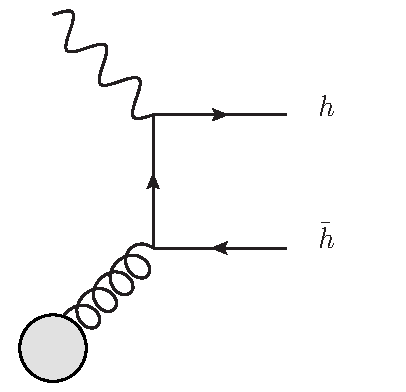
\includegraphics[scale=0.6]{2-PDFs/figs/FFNS.pdf}
\end{figure}

This approach is known as the \emph{decoupling} or FFN scheme where the only quarks treated as partons are the $n_l$ light quarks. The expression in Eqn.~\ref{eq:FFN} is unique up to terms of order $m_l^2/Q^2$ in the light quark masses which are typically treated as part of the factorisation level corrections of $\mathcal{O}(\Lambda^2_{\mathrm{QCD}}/Q^2)$. While accurate in the quark mass threshold region and below, this scheme suffers from unresummed logarithms of the ratio $Q^2/m_h^2$ contained in the Wilson coefficients which can become large and damage the convergence of the perturbative series at scales much larger than the heavy quark mass.

These problems may be resolved in a scheme which treats the heavy quark as a massless parton above its mass threshold with the introduction of an associated heavy quark PDF. The subsequent renormalisation of the PDF resums the logarithmic contributions due to parton splitting via solution of the DGLAP equation, removing a significant disadvantage present in the FFN treatment. As this scheme is identical to the zero mass scheme discussed previously, but with an additional partonic flavour, this procedure is known as the Zero-Mass Variable Flavour Number (ZM-VFN) scheme. In the ZM-VFN a structure function calculation is simply

\be F(n_l+1, x,Q^2) = \sum_i^{n_l+1} C_i\left(n_l+1,\frac{Q^2}{\mu^2} \right) \otimes f_i(n_l+1,\mu^2). \label{eq:ZMVFN} \ee
In this instance the heavy quark contribution to the structure function first arises now at leading order via diagrams of the type:

\begin{figure}[h]
\centering
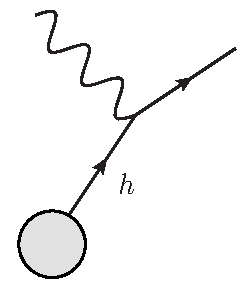
\includegraphics[scale=0.6]{2-PDFs/figs/ZMVFNS.pdf}
\end{figure}

In the ZM-VFNS the heavy quark PDFs are set to zero below mass threshold and evolved as a massless parton according to the DGLAP equations for scales greater than the heavy quark mass. While this method alleviates the difficulties present in the FFN scheme at large scales, its treatment of heavy quarks only in terms of massless partons completely ignores the massive contributions to the Wilson coefficients and is therefore no longer exact. The reliability of the ZM scheme is therefore particularly reduced in the region where powers of $m_h^2/Q^2$ are significant. 
\subsection{General mass schemes}
Analyses of QCD measurements are often performed by making a choice between using a suitable FFN scheme at scales in the region of heavy quark mass thresholds or a ZM scheme at high scales where the associated powers of $m_h^2/Q^2$ can be safely neglected. In either case the treatment of heavy quarks is at least unambiguous, with the ZM approach yielding a simpler procedure as there is no requirement to calculate coefficient functions with the heavy quark masses intact.

For analyses of a large dataset, potentially spanning several heavy quark thresholds and extending to very high scales, the desire to improve the perturbative reliability of the calculations has led to the development of a number of hybrid or \emph{general mass} schemes. In such schemes the treatments generally reduce to the FFN regime at low scales and the ZM treatment at high scales, with the intermediate regime handled via some interpolation between the two. Generally in a Variable Flavour Number (VFN) scheme one requires that
\be F^{L}(n_l, Q^2) + \lim_{Q^2 \gg m_h^2} \left[ F^{H}(n_l, Q^2,m_h^2)\right] =  F(n_l+1, x,Q^2), \label{eq:VFN}\ee
i.e. that the ZM-VFN and FFN calculations coincide at large scales, where the heavy quark mass dependance of the FFN Wilson coefficients can be neglected. The constraint in Eqn. \ref{eq:VFN} means that parton distributions in the two schemes may be related by a perturbatively calculable transformation.

\be f_i(n_l+1,\mu^2) = \sum_j^{n_l}A_{ij}\left(n_l, \frac{\mu^2}{m_h^2}\right)\otimes f_j(n_l, \mu^2), \label{eq:FLVreln}\ee
where the $A$ are determined to NNLO in $\alpha_S$ in Refs.~\cite{Buza:1995ie,Buza:1996wv}. It should be noted that the $A$ are not square matrices, with $i$ running over the $n_l+1$ partons in the zero mass scheme, and the $j$ running over the $n_l$ partons in the FFN.

In general a GM-VFN operates as a tower of FFN-type schemes with increasing $n_l$ as the scale increases over each quark mass threshold. In constructing a GM-VFN, the guiding principle is that physical observables should be continuous across these thresholds and therefore continuous across the $n_l$ and $n_l+1$ regimes. 
Taking the heavy quark mass itself as the matching point between the two regimes, we demand that the GM-VFN structure function $F^{\text{GM}}$ obeys
\ba 
F^{\text{GM}}(m_h^2) &=& \sum_j^{n_l} C^{\text{GM}}_j \left(n_l, m_h^2 \right) \otimes f_j(n_l) \nonumber \\
&=&   \sum_i^{n_l+1} C^{\text{GM}}_i\left( n_l+1, m_h^2 \right) \otimes f_i(n_l+1). \label{eq:GMmatching} 
\ea 
where the dependance upon the perturbative scales has been omitted for notational simplicity, and the GM superscripts refer to the coefficients in a general mass scheme. Using the relation in Eqn. \ref{eq:FLVreln} we can express the $n_l+1$ expression in the matching Eqn. \ref{eq:GMmatching} in terms of the $n_l$ scheme PDFs, therefore obtaining the relation
\ba && \sum_j^{n_l} C^{\text{GM}}_j \left(n_l, m_h^2 \right) \otimes f_j(n_l) \\
=  && \sum_i^{n_l+1} \sum_j^{n_l } C^{\text{GM}}_i\left( n_l+1, m_h^2 \right) \otimes A_{ij}\left(n_l, m_h^2\right)\otimes f_j(n_l). \ea
Subsequently, we may make the identification
\be  C^{\text{GM}}_j \left(n_l, m_h^2 \right) 
=   \sum_i^{n_l+1} C^{\text{GM}}_i\left( n_l+1,m_h^2 \right) \otimes A_{ij}\left(n_l, m_h^2\right),\label{eq:minimalGM}\ee
which provides the minimal description for the construction of a GM-VFN scheme~\cite{Thorne:2008xf}. Ensuring that Eqn.~\ref{eq:minimalGM} is satisfied order by order in $\alpha_S$, we can construct the expression for the GM-VFN scheme coefficient functions above the heavy quark mass threshold. Taking the simplistic example case of Ref.~\cite{Kramer:2000hn} with a theory including only a gluon and a single heavy quark ($h=\bar{h}$), the GM-VFN coefficients may be constructed to order $\alpha_S$ as
\ba
C_g^{\text{LO}}(n_l+1,m_h) &=& C_g^{\text{LO}}(n_l,m_h), \\
C_g^{\text{NLO}}(n_l+1,m_h) &=& C_g^{\text{NLO}}(n_l,m_h) \nonumber \\
&-& C_h^{\text{LO}}(n_l+1,m_h)\otimes A^{\text{LO}}_{hg}(n_l, m_h^2). \label{eq:ACOT}
\ea
where the GM superscript has been omitted, the new superscript specifying the order of the term in the perturbative expansions of the quantities $C$ and $A$. Here the rightmost term in the $\mathcal{O}(\alpha_S)$ expression Eqn.~\ref{eq:ACOT} is known as the \emph{subtraction term} which ensures the cancellation of the IR-unsafe scale logs present in the FFN calculation. The ambiguity in the definition of a GM-VFNS arises upon noticing that terms proportional to powers of $m_h/Q$ may be interchanged between the Wilson coefficients in Eqn.~\ref{eq:ACOT} without changing the final value of the structure function. In this respect changing the distribution of terms between the gluon and heavy quark initiated diagrams in Eqn.~\ref{eq:ACOT} provides the opportunity to perform a \emph{scheme choice}, a freedom which has been exploited by several different GM-VFN scheme implementations. 

The earliest complete description of a GM-VFNS was provided by the ACOT method~\cite{Collins:1978wz} which ensures the continuity of physical quantities through Eqn.~\ref{eq:minimalGM}, but does not attempt to take advantage of the degeneracy in the GM-VFN procedure. An important result was achieved with the Simplified-ACOT or S-ACOT  scheme~\cite{Collins:1998rz,Kramer:2000hn} which was able to exploit this ambiguity to considerably simplify the calculation of physical observables. In the S-ACOT scheme it was noted that shifts of the Wilson coefficients by their zero-mass limits may be absorbed into a redefinition of the GM-VFNS. That is, terms such as
\be C_h(n_l+1, m_h) - C_h(n_l+1, 0),\ee
vanish in the limit $Q^2 \gg m_h^2$, and therefore do not spoil the interpolation between the FFN and ZM schemes. This leads to the option of shifting to a simpler scheme where the massive heavy quark initiated coefficients may instead be evaluated with the heavy quark mass set to zero. Other options for the scheme definition were explored by Thorne and Roberts in the TR type schemes~\cite{Thorne:1997uu,Thorne:1997ga}, with the additional constraint that scale derivatives of heavy flavour structure functions should also be continuous at the matching scale.
%
\subsubsection{The FONLL approach}
%
A more recent approach was developed by examining methods previously used to combine fixed order calculations with next-to-leading log resummation via the FONLL method~\cite{Cacciari:1998it}. The method was extended from the original application of studying the \pt spectrum in heavy flavour hadroproduction to the treatment of heavy quarks in DIS by Forte \emph{et al.}~\cite{Forte:2010ta}. The procedure begins by inverting the relationship in Eqn.~\ref{eq:FLVreln} so as to express an $n_l$ flavour structure function in terms of $n_l+1$ flavour PDFs,
\be F(n_l,Q^2) = \sum_i^{n_l} B_i\left(\frac{Q^2}{m_h^2}\right)\otimes f_i(n_l+1,Q^2), \label{eq:FONLLmassive}\ee
where it is important to note that the sum over flavours does not include the heavy flavour PDF, and the full heavy quark mass dependence is present in the coefficients $B$. To perform a matching with the massless scheme, the ZM result in Eqn.~\ref{eq:ZMVFN} can be expressed in terms of light flavour PDFs only, given the assumption that the heavy flavour PDF is generated perturbatively. In this case, Eqn.~\ref{eq:ZMVFN} can be written
\be F(n_l+1, Q^2) = \sum_i^{n_l} \widetilde{C}_i\left(n_l+1,\frac{Q^2}{m_h^2} \right) \otimes f_i(n_l+1,\mu^2). \label{eq:FONLLmassless}\ee
where once again, the sum runs over only light flavours, this time with the heavy flavour contribution being generated via DGLAP evolution included into the modified coefficient function $\widetilde{C}$. To understand which terms are common in the two descriptions, the massive coefficient functions may be decomposed into terms logarithmically dependant upon the heavy quark mass, and terms suppressed by powers of $m_h/Q$: 
\be B_i\left(\frac{Q^2}{m_h^2}\right) = \overline{B}_i\left(\frac{Q^2}{m_h^2}\right) + \mathcal{O}\left(\frac{m_h}{Q}\right).\ee  
As only the power suppressed terms vanish in the limit of $Q^2 \gg m_h^2$, the terms remaining must be common to both the ZM and massive scheme calculations. We can therefore express the massive structure function in a `\emph{massless}' limit, having dropped those terms in the coefficient functions that are suppressed by powers of $m_h/Q$:
\be \overline{F}(n_l,Q^2) = \sum_i^{n_l} \overline{B}_i\left(\frac{Q^2}{m_h^2}\right)\otimes f_i(n_l+1,Q^2).\label{eq:FONLLdoublecount}\ee
The FONLL result for the structure function is given by the sum of the massive calculation in Eqn.~\ref{eq:FONLLmassive}, and the massless calculation in Eqn.~\ref{eq:FONLLmassless} with the asymptotic limit of the massive calculation in Eqn.~\ref{eq:FONLLdoublecount} subtracted. 
\be
F^{\mathrm{FONLL}}(Q^2) =\left[ F(n_l,Q^2) + F(n_l+1, Q^2) \right] - \overline{F}(n_l,Q^2).
\ee
With the subtraction ensuring the cancellation of terms which are double counted between the massive and massless calculations. Therefore in this expression the mass-suppressed terms present in the FFN calculation are fully accounted for in the GM scheme, with the duplicate terms subtracted. The simplicity of this approach helped to elucidate many of the differences between general mass schemes.

It should be noted that while general mass schemes suffer from an ambiguity in their definition compared to the simpler fixed-flavour and zero mass schemes, the differences between them are always of higher order compared to the calculation at hand, as is the case in any true scheme choice. Indeed, a well-defined GM-VFNS will always reduce to the decoupled result at low scales and the zero-mass result at scales much higher than the quark mass, behaving effectively as a tower of fixed flavour schemes with increasing number of partonic quarks. The general-mass schemes therefore do not suffer from a significant loss of predictive power, and are able to provide considerable improvement over the simpler schemes when dealing with datasets spanning quark mass thresholds.
%
\section{General features of parton distributions}
%
While we have now described how the parton distributions functions at an experimental scale $Q^2$ may be found by evolving parton distributions from an initial scale, and discussed briefly how the renormalisation of heavy quark distributions may be accomplished, the issue of determining the functional dependence of the parton distributions upon the momentum fraction $x$ at some initial scale $f_i(x,Q_0^2)$ remains. 

The number of independent PDFs to be determined is dependent upon the choice of initial scale, as quark distributions that can be considered \emph{heavy} with respect to $Q^2_0$ may be generated perturbatively through the DGLAP procedure outlined previously. The typical choice is to determine the parton distributions at some scale $ m_s^2< Q^2_0 \le m_c^2$ such that the flavours $c$, $b$, $t$ are produced by evolution. These scale choices minimise the number of distributions to be determined while remaining perturbatively reliable.

As the remaining seven distributions\footnote{The gluon, the $u$, $d$, $s$ quarks and their antiquarks.} are fundamentally a parametrisation of the nonperturbative dynamics of the proton, they are by definition out of reach of a perturbative analysis. There are however some general statements that may be made of their $x$-dependence that are independent of the hard scale. The most important of which are the parton distribution \emph{sum rules} which constrain the relative normalisation of PDFs.

Firstly, the \emph{momentum sum rule} (MSR) ensures that the parton distributions' fractional momenta sum to the momentum of the parent proton
\be  \int_0^1 dx \left[  x\Sigma(x,Q^2) + xg(x,Q^2) \right]= 1, \label{eq:MSR} \ee
where $\Sigma$ is the singlet distribution defined previously. Following this are the quark valence sum rules. These fix the quark distributions such that the resulting proton has the appropriate quantum numbers,
\begin{subequations}
\label{eq:VSR}
\ba \text{up-valence:}& \: &\int_0^1 dx\left( f_u(x,Q^2) - f_{\bar{u}}(x,Q^2) \right) = 2, \label{eq:UVSR} \\
      \text{down-valence:}&  \: & \int_0^1 dx\left( f_d(x,Q^2) - f_{\bar{d}}(x,Q^2) \right) = 1, \label{eq:DVSR}\\
      \text{strange-valence:}&  \: & \int_0^1 dx\left( f_s(x,Q^2) - f_{\bar{s}}(x,Q^2) \right) = 0. \label{eq:SVSR} 
\ea
\end{subequations}

From these rules we may infer additional constraints upon individual PDFs. The MSR suggests a form for the large-$x$ behaviour of the distributions, in that they should parametrically tend to zero as $x\to1$. The number sum rules in Eqns. \ref{eq:VSR} require the valence-type distributions to be integrable over the whole $x$-range. While there is no requirement for the singlet and gluon distributions to be integrable, their first moments must be, as required by the MSR. Combining these three constraints we may parametrise the large and small-$x$ behaviour of both valence-like and gluon or singlet-like distributions as:
\ba f_V(x,Q_0^2) &= N_V\;x^{\alpha_V}(1-x)^{\beta_V}\,r_V(x), \nonumber \\
 f_\Sigma(x,Q_0^2) &= N_\Sigma\;x^{\alpha_\Sigma}(1-x)^{\beta_\Sigma}\,r_\Sigma(x). \label{eq:pdflimits}\ea
In these expressions, the parameters $\alpha$ and $\beta$ control the small and large-$x$ PDF behaviour respectively. The $\beta$ should be such that the PDFs tend to zero smoothly at large-$x$, and the $\alpha$ such that the valence distributions are integrable, and the first moment of the gluon and singlet are integrable. The overall PDF normalisations $N$ being constrained via the appropriate sum rules.

Finally, what remains in the determination of the distributions are the remainder terms $r(x)$ which describe the PDFs between the two $x$-limits. Their determination is considerably more complex and is a ongoing source of research. Much of this thesis will be dedicated to discussing the determination of these remainder functions.